\documentclass[12pt]{beamer}

%%%%%%%%%%%%%%%%%%%%%%%%%%%%%%%%%%%%%%%%%%%%%%%%%%%%%%%%%%%%%%%%%%%%%%%%%%%%%%%%
% LaTeX Imports
%%%%%%%%%%%%%%%%%%%%%%%%%%%%%%%%%%%%%%%%%%%%%%%%%%%%%%%%%%%%%%%%%%%%%%%%%%%%%%%%
\usepackage{amsfonts}                                                   % Math fonts
\usepackage{amsmath}                                                    % Math formatting
\usepackage{amssymb}                                                    % Math formatting
\usepackage{amsthm}                                                     % Math Theorems
\usepackage{arydshln}                                                   % Dashed hlines
\usepackage{attachfile}                                                 % AttachFiles
\usepackage{cancel}                                                     % Cancelled math
\usepackage{caption}                                                    % Figure captioning
\usepackage{color}                                                      % Nice Colors
\input{./lib/dragon.inp}                                                % Tikz dragon curve
\usepackage[ampersand]{easylist}                                        % Easy lists
\usepackage{fancyhdr}                                                   % Fancy Header
\usepackage[T1]{fontenc}                                                % Specific font-encoding
%\usepackage[margin=1in, marginparwidth=2cm, marginparsep=2cm]{geometry} % Margins
\usepackage{graphicx}                                                   % Include images
\usepackage{hyperref}                                                   % Referencing
\usepackage[none]{hyphenat}                                             % Don't allow hyphenation
\usepackage{lipsum}                                                     % Lorem Ipsum Dummy Text
\usepackage{listings}                                                   % Code display
\usepackage{marginnote}                                                 % Notes in the margin
\usepackage{microtype}                                                  % Niceness
\usepackage{lib/minted}                                                 % Code display
\usepackage{multirow}                                                   % Multirow tables
\usepackage{pdfpages}                                                   % Include pdfs
\usepackage{pgfplots}                                                   % Create Pictures
\usepackage{rotating}                                                   % Figure rotation
\usepackage{setspace}                                                   % Allow double spacing
\usepackage{subcaption}                                                 % Figure captioning
\usepackage{tikz}                                                       % Create Pictures
\usepackage{tocloft}                                                    % List of Equations
%%%%%%%%%%%%%%%%%%%%%%%%%%%%%%%%%%%%%%%%%%%%%%%%%%%%%%%%%%%%%%%%%%%%%%%%%%%%%%%%
% Package Setup
%%%%%%%%%%%%%%%%%%%%%%%%%%%%%%%%%%%%%%%%%%%%%%%%%%%%%%%%%%%%%%%%%%%%%%%%%%%%%%%%
\hypersetup{%                                                           % Setup linking
    colorlinks=true,
    linkcolor=black,
    citecolor=black,
    filecolor=black,
    urlcolor=black,
}
\RequirePackage[l2tabu, orthodox]{nag}                                  % Nag about bad syntax
\renewcommand*\thesection{\arabic{section} }                             % Reset numbering
\renewcommand{\theFancyVerbLine}{ {\arabic{FancyVerbLine} } }              % Needed for code display
\renewcommand{\footrulewidth}{0.4pt}                                    % Footer hline
\setcounter{secnumdepth}{3}                                             % Include subsubsections in numbering
\setcounter{tocdepth}{3}                                                % Include subsubsections in toc
%%%%%%%%%%%%%%%%%%%%%%%%%%%%%%%%%%%%%%%%%%%%%%%%%%%%%%%%%%%%%%%%%%%%%%%%%%%%%%%%
% Custom commands
%%%%%%%%%%%%%%%%%%%%%%%%%%%%%%%%%%%%%%%%%%%%%%%%%%%%%%%%%%%%%%%%%%%%%%%%%%%%%%%%
\newcommand{\nvec}[1]{\left\langle #1 \right\rangle}                    %  Easy to use vector
\newcommand{\ma}[0]{\mathbf{A} }                                         %  Easy to use vector
\newcommand{\mb}[0]{\mathbf{B} }                                         %  Easy to use vector
\newcommand{\abs}[1]{\left\lvert #1 \right\rvert}                       %  Easy to use abs
\newcommand{\pren}[1]{\left( #1 \right)}                                %  Big parens
\let\oldvec\vec
\renewcommand{\vec}[1]{\oldvec{\mathbf{#1} } }                            %  Vector Styling
\newtheorem{thm}{Theorem}                                               %  Define the theorem name
\newtheorem{definition}{Definition}                                     %  Define the definition name
\definecolor{bg}{rgb}{0.95,0.95,0.95}
\newcommand{\java}[4]{\vspace{10pt}\inputminted[firstline=#2,
                                 lastline=#3,
                                 firstnumber=#2,
                                 gobble=#4,
                                 frame=single,
                                 label=#1,
                                 bgcolor=bg,
                                 linenos]{java}{#1} }
\newcommand{\python}[4]{\vspace{10pt}\inputminted[firstline=#2,
                                 lastline=#3,
                                 firstnumber=#2,
                                 gobble=#4,
                                 frame=single,
                                 label=#1,
                                 bgcolor=bg,
                                 linenos]{python}{#1} }
\newcommand{\js}[4]{\vspace{10pt}\inputminted[firstline=#2,
                                 lastline=#3,
                                 firstnumber=#2,
                                 gobble=#4,
                                 frame=single,
                                 label=#1,
                                 bgcolor=bg,
                                 linenos]{js}{#1} }
%%%%%%%%%%%%%%%%%%%%%%%%%%%%%%%%%%%%%%%%%%%%%%%%%%%%%%%%%%%%%%%%%%%%%%%%%%%%%%%%
% Beginning of document items - headers, title, toc, etc...
%%%%%%%%%%%%%%%%%%%%%%%%%%%%%%%%%%%%%%%%%%%%%%%%%%%%%%%%%%%%%%%%%%%%%%%%%%%%%%%%
\pagestyle{fancy}                                                       %  Establishes that the headers will be defined
\fancyhead[LE,LO]{Computer Systems Notes}                                  %  Adds header to left
\fancyhead[RE,RO]{Zoe Farmer}                                       %  Adds header to right
\cfoot{ \thepage }
\lfoot{CSCI 2400}
\rfoot{Han}
\title{Computer Systems Notes}
\author{Zoe Farmer}

\usepackage{multimedia}
%%%%%%%%%%%%%%%%%%%%%%%%%%%%%%%%%%%%%%%%%%%%%%%%%%%%%%%%%%%%%%%%%%%%%%%%%%%%%%%%
% Beginning of document items - headers, title, toc, etc...
%%%%%%%%%%%%%%%%%%%%%%%%%%%%%%%%%%%%%%%%%%%%%%%%%%%%%%%%%%%%%%%%%%%%%%%%%%%%%%%%
\title[PACE]{Parameterization and Analysis of Viscous Fluid Conduit Edges for
    Dispersive Hydrodynamics}
    \author{Zoe Farmer\\\url{www.dataleek.io}}
\institute{University of Colorado, Boulder\\
            Advisors: Mark Hoefer, Michelle Maiden}
\date{March 5, 2016}


%%%%%%%%%%%%%%%%%%%%%%%%%%%%%%%%%%%%%%%%%%%%%%%%%%%%%%%%%%%%%%%%%%%%%%%%%%%%%%%%
% Custom Beamer Theming
%%%%%%%%%%%%%%%%%%%%%%%%%%%%%%%%%%%%%%%%%%%%%%%%%%%%%%%%%%%%%%%%%%%%%%%%%%%%%%%%
\usetheme{Madrid}
\makeatletter

% http://tex.stackexchange.com/questions/35166/how-can-i-remove-the-institute-from-the-author-footline-on-beamer
% TLDR; Remove the Institution from default Madrid theme by redefining footline
% template.
\setbeamertemplate{footline}
{
  \leavevmode%
  \hbox{%
  \begin{beamercolorbox}[wd=.333333\paperwidth,ht=2.25ex,dp=1ex,center]{author in head/foot}%
      \usebeamerfont{author in head/foot}{\color{cugold}\insertshortauthor}%~~\beamer@ifempty{\insertshortinstitute}{}{(\insertshortinstitute)}
  \end{beamercolorbox}%
  \begin{beamercolorbox}[wd=.333333\paperwidth,ht=2.25ex,dp=1ex,center]{title in head/foot}%
    \usebeamerfont{title in head/foot}\insertshorttitle
  \end{beamercolorbox}%
  \begin{beamercolorbox}[wd=.333333\paperwidth,ht=2.25ex,dp=1ex,right]{date in head/foot}%
    \usebeamerfont{date in head/foot}\insertshortdate{}\hspace*{2em}
    \insertframenumber{} / \inserttotalframenumber\hspace*{2ex} 
  \end{beamercolorbox}}%
  \vskip0pt%
}
\makeatother

% Redefine title page to be a little more square/2d
\setbeamertemplate{title page}
{
  \begin{centering}
    \begin{beamercolorbox}[sep=8pt,center]{title}
      \usebeamerfont{title}\inserttitle\par%
      \ifx\insertsubtitle\@empty%
      \else%
        \vskip0.25em%
        {\usebeamerfont{subtitle}\usebeamercolor[fg]{subtitle}\insertsubtitle\par}%
      \fi%     
    \end{beamercolorbox}%
    \begin{beamercolorbox}[sep=8pt,center]{institute}
      \usebeamerfont{institute}\insertinstitute
    \end{beamercolorbox}
    \vskip1em\par
    \begin{beamercolorbox}[sep=8pt,center]{date}
      \usebeamerfont{date}\insertdate
    \end{beamercolorbox}%\vskip0.5em
    \begin{beamercolorbox}[sep=8pt,center]{author}
      \usebeamerfont{author}\insertauthor
    \end{beamercolorbox}
  \end{centering}
  %\vfill
}
\makeatother

\usecolortheme{wolverine}

%%%%% SET THEME
\beamertemplatenavigationsymbolsempty   % Disable navigation

%%%%% INSERT LOGO
\logo{%
    \vspace{-0.3cm}
    \makebox[0.95\paperwidth]{%
        
\includegraphics[scale=0.4]{./img/nsf.png}{\color{cublack}Funded by NSF EXTREEMS-QED}
        \hfill%
        \color{cugold}CU Boulder Applied Math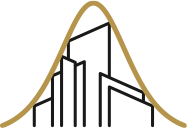
\includegraphics[height=0.8cm]{./img/appm.png}
    }%
}

%%%%% DEFINE COLORS
\definecolor{bgcolor}{RGB}{255,255,240}
\definecolor{cugold}{RGB}{207,184,124}
\definecolor{cublack}{RGB}{0,0,0}
\definecolor{cudarkgray}{RGB}{86,90,92}
\definecolor{culightgray}{RGB}{162,164,163}

%%%%% SET COLORS
\setbeamercolor{palette primary}{bg=cugold,fg=cublack}
\setbeamercolor{palette secondary}{bg=culightgray}
\setbeamercolor{palette tertiary}{bg=cublack}
\setbeamercolor{frametitle}{bg=cugold,fg=cublack}
\setbeamercolor{item projected}{fg=cugold,bg=black}
\setbeamercolor{itemize item}{fg=cublack,bg=black}

%%%%% List Styling
\setbeamertemplate{itemize items}[circle]
\setbeamertemplate{enumerate items}[circle]

%%%%%%%%%%%%%%%%%%%%%%%%%%%%%%%%%%%%%%%%%%%%%%%%%%%%%%%%%%%%%%%%%%%%%%%%%%%%%%%%
% Document
%%%%%%%%%%%%%%%%%%%%%%%%%%%%%%%%%%%%%%%%%%%%%%%%%%%%%%%%%%%%%%%%%%%%%%%%%%%%%%%%
\begin{document}
\frame{\titlepage}

\logo{%
    \vspace{-0.3cm}\color{cugold}CU Boulder Applied Math
    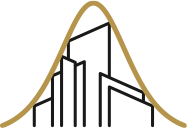
\includegraphics[height=0.8cm]{./img/appm.png}
}

\frame{%
    \frametitle{Dispersive Hydrodynamics Lab}
    Our lab has four main facets
    \begin{enumerate}
        \item Experimental Observations
        \item Analytical Solutions
        \item Numerical Solutions
        \item Data Analysis (part of the NSF EXTREEMS-QED program)
    \end{enumerate}

    In order to have accurate results, we need to make sure we have accurate
    data.\vspace{0.5cm}

    \textbf{Poor quality data yields poor quality results.}
}

\frame{%
    \frametitle{High Level Overview}
    \begin{columns}[T]
        \column{0.5\textwidth}
        \begin{itemize}
            \item In our lab we examine the dynamics of a viscous fluid conduit.
            \item One large issue is that sometimes the conduits that are formed
                curve, and spiral around a central axis.
            \item We determine a method to measure the degree of spiraling, and
                to reject conduits based on this degree.
        \end{itemize}
        \column{0.5\textwidth}
        \begin{figure}[H]
            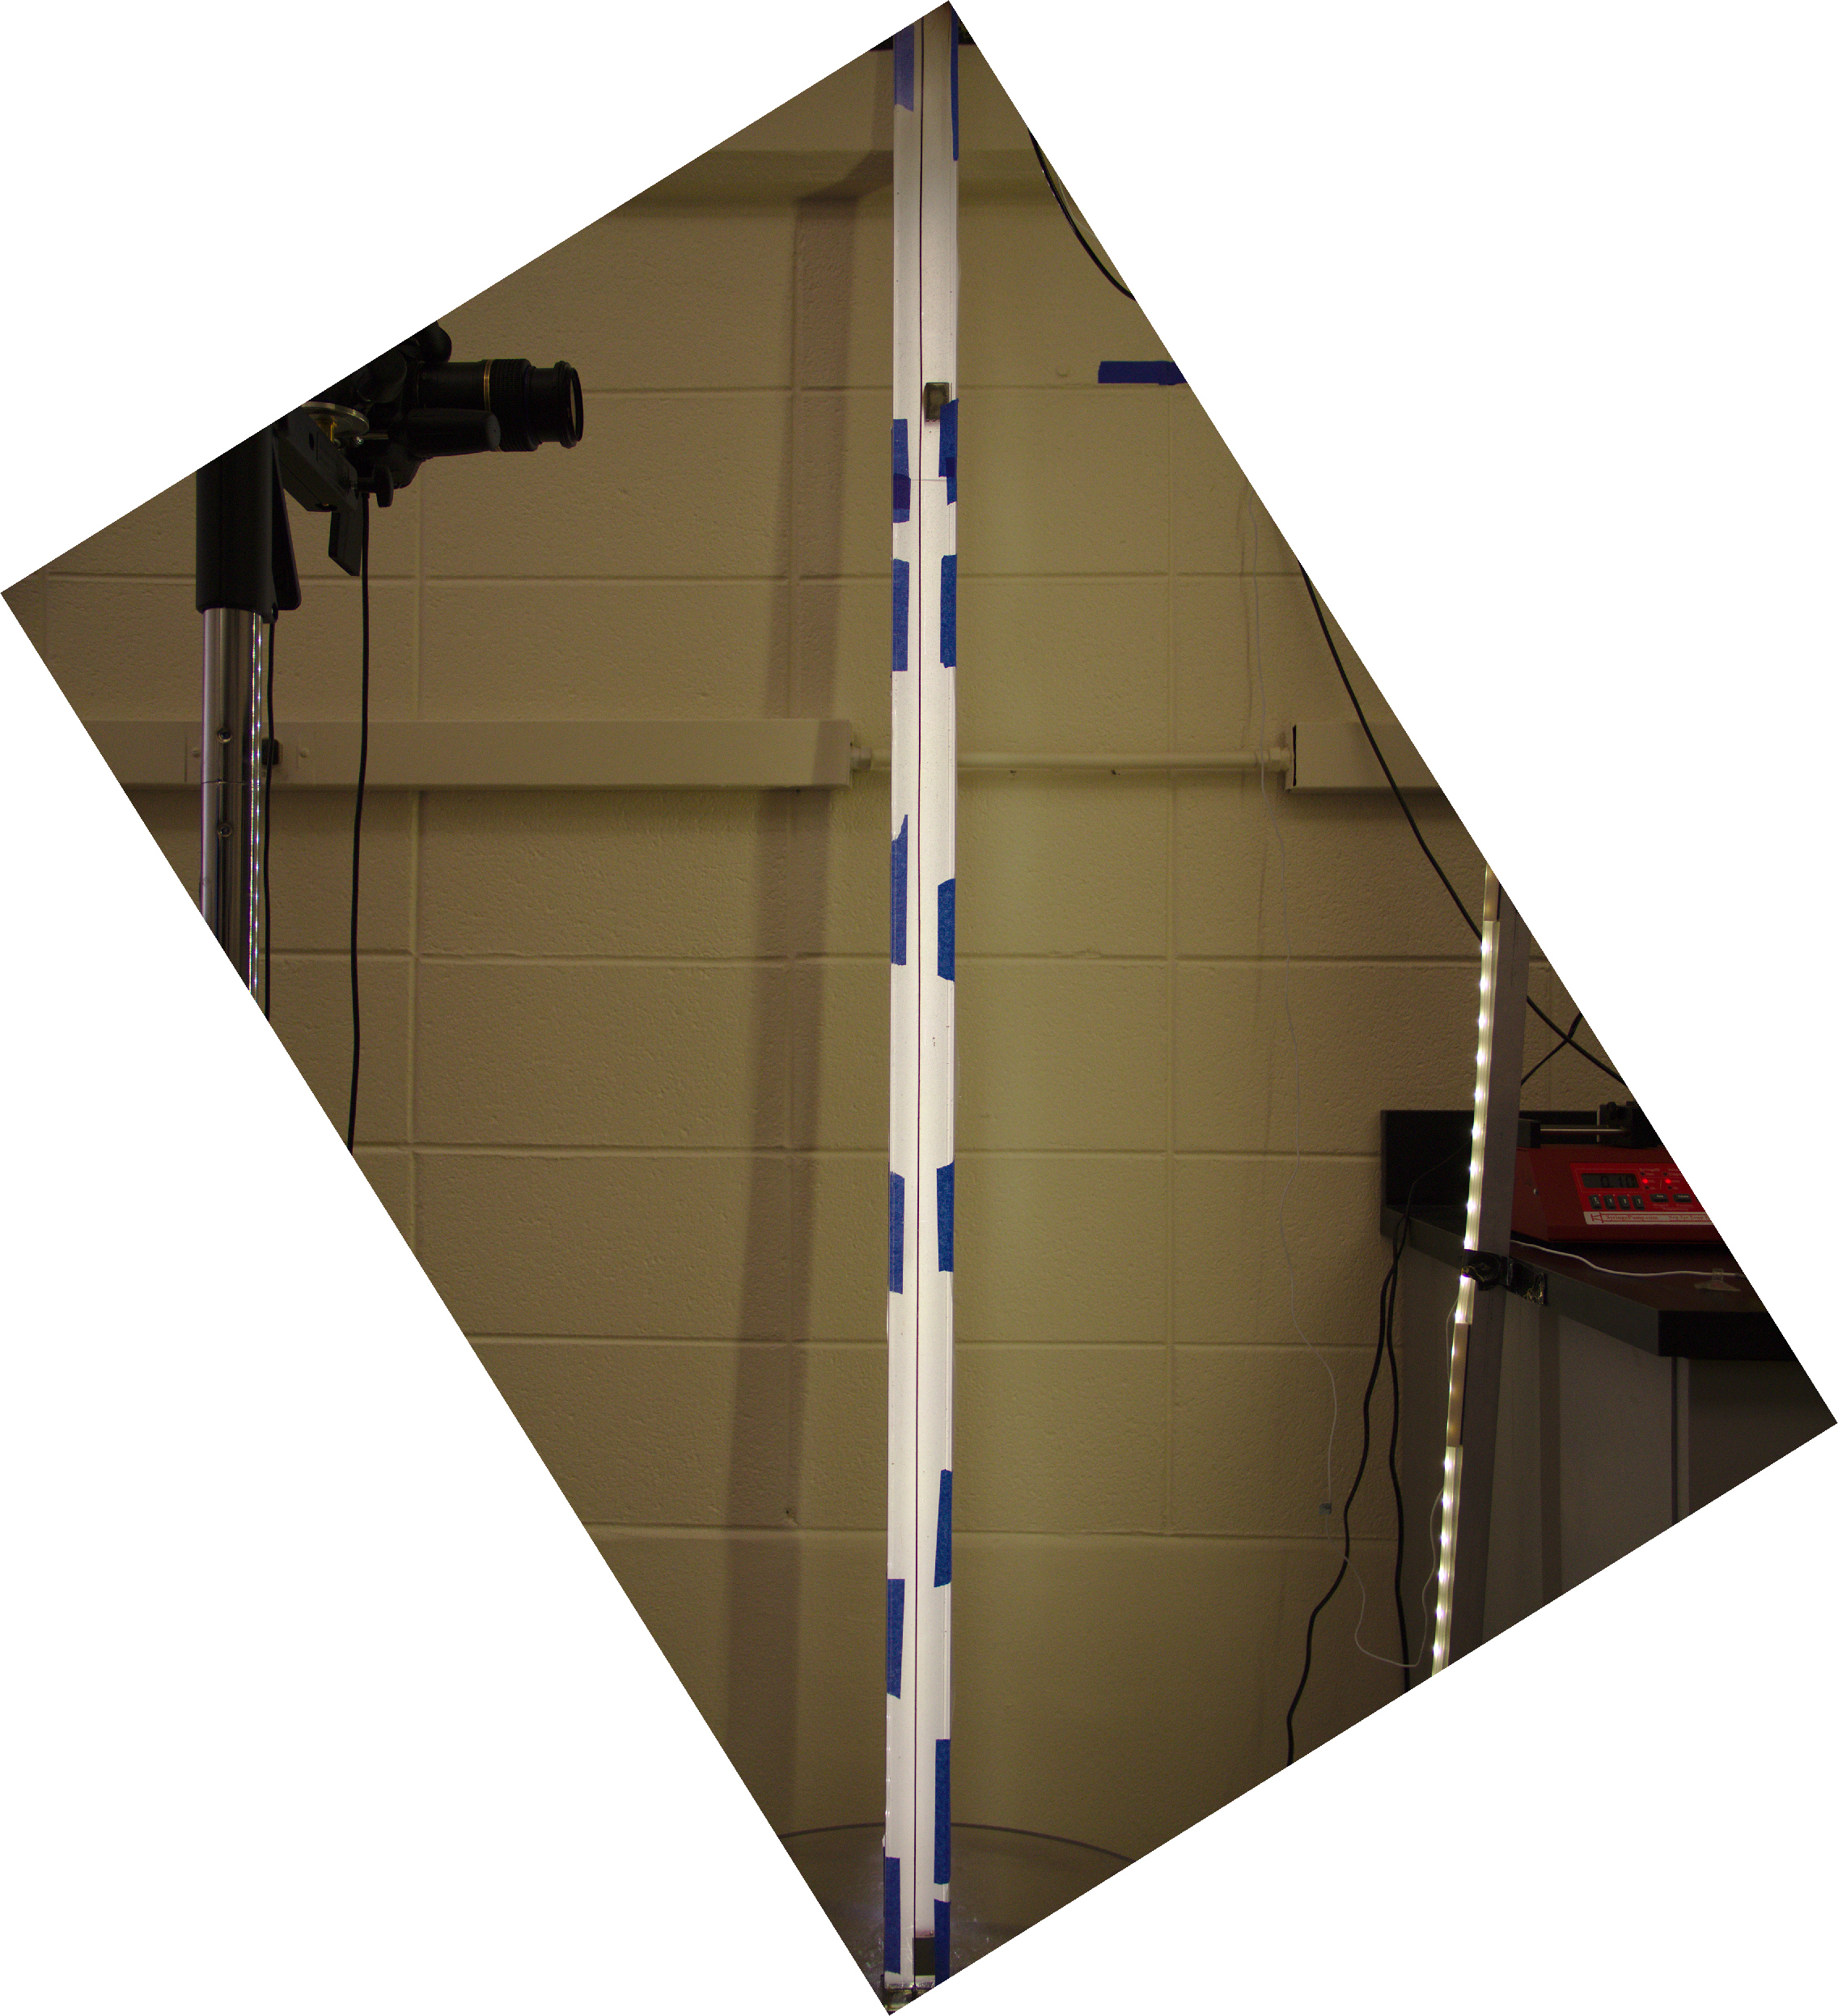
\includegraphics[scale=0.065]{./img/final.png}
        \end{figure}
    \end{columns}
    This is a \textbf{Data Quality Problem}.
}

\frame{%
    \frametitle{What's our Environment?}
    \begin{columns}[T]
        \column{0.5\textwidth}
        \textbf{Viscous Fluid Conduits}
        \begin{itemize}
            \item Two viscous fluids, with inner forming axisymmetric conduit.
            \item Exterior Fluid: $\rho^{(e)}$ density and $\mu^{(e)}$ viscosity
            \item Interior Fluid: $\rho^{(i)}$ density and $\mu^{(i)}$ viscosity
            \item $\rho^{(i)} < \rho^{(e)} \Rightarrow$ buoyant flow
            \item $\mu^{(i)} << \mu^{(e)} \Rightarrow$ minimal drag
            \item $\text{Re} << 1 \Rightarrow$ low Reynold's number
        \end{itemize}
        \column{0.5\textwidth}
        \begin{figure}[H]
            \centering
            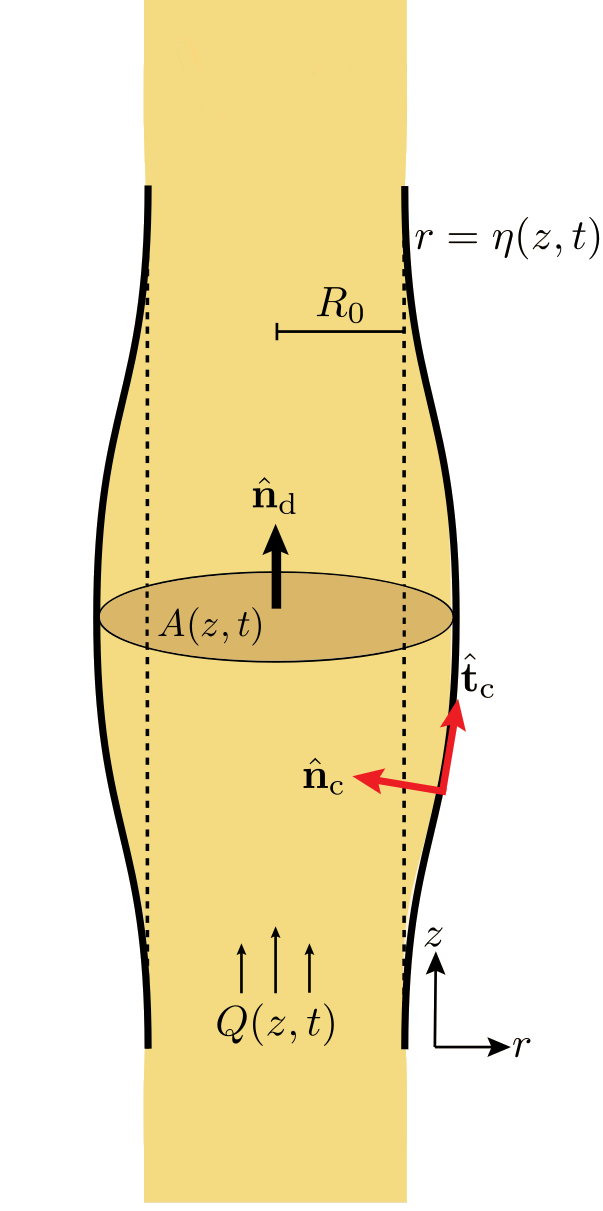
\includegraphics[scale=0.15]{./img/conduit.png}
        \end{figure}
    \end{columns}
}

\frame{%
    \frametitle{Experimental Setup}
    \begin{figure}[H]
        \centering
        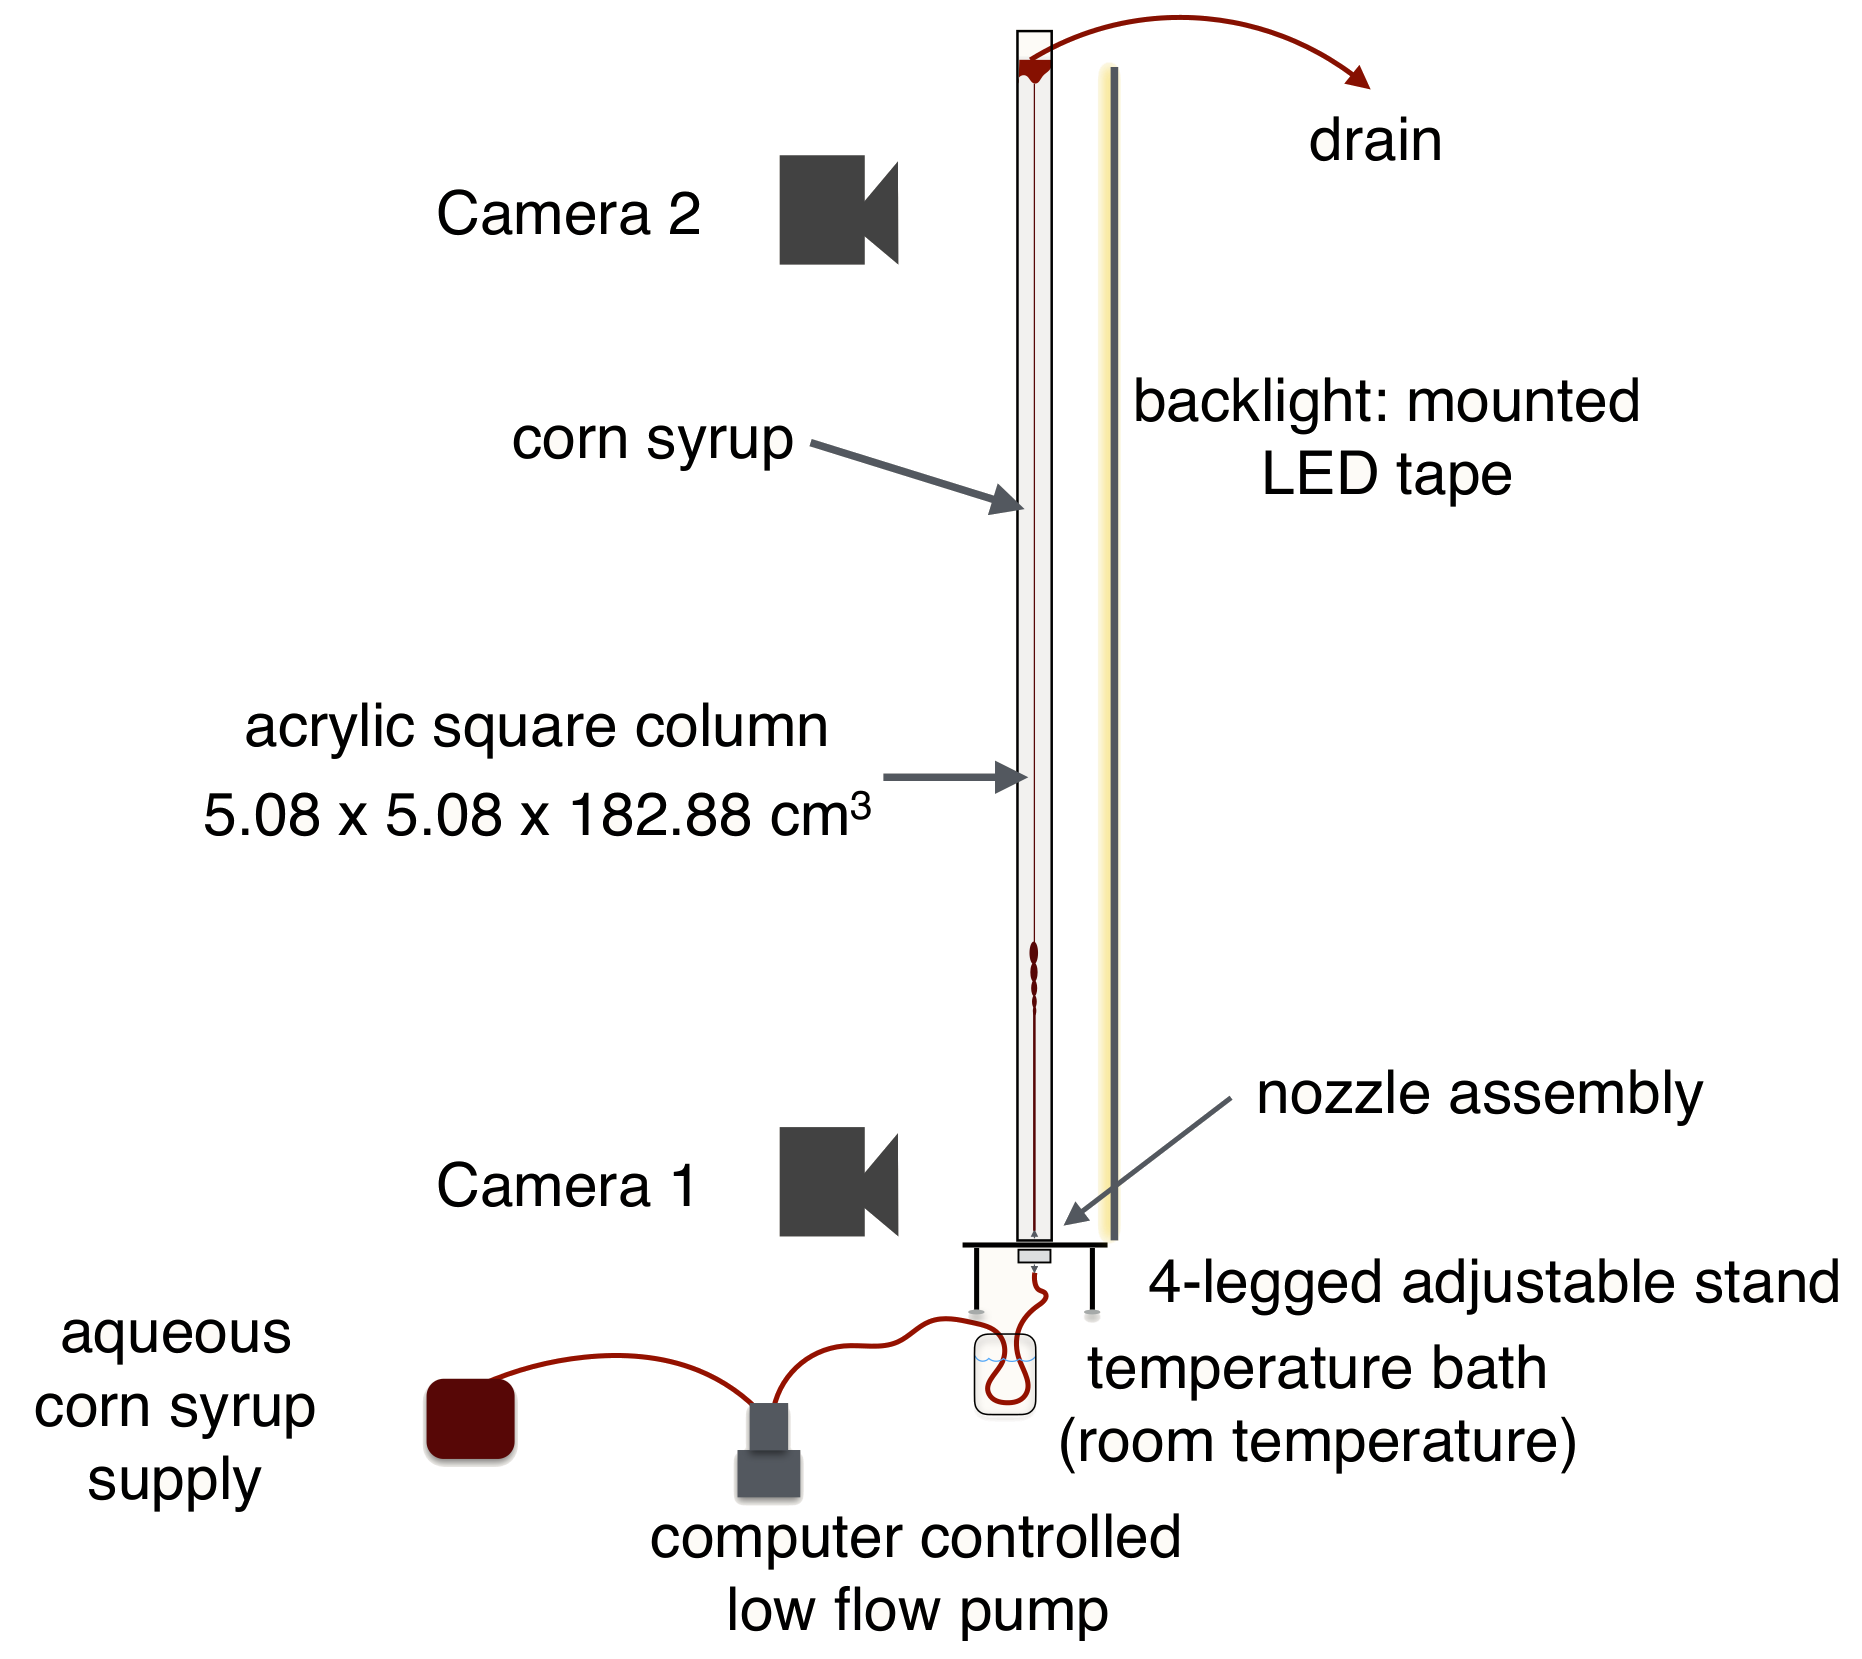
\includegraphics[scale=0.13]{./img/setup.png}
    \end{figure}
}

\frame{%
    \frametitle{Data Collection}
    \begin{columns}[T]
        \column{0.33\textwidth}
        \begin{figure}[H]
            \centering
            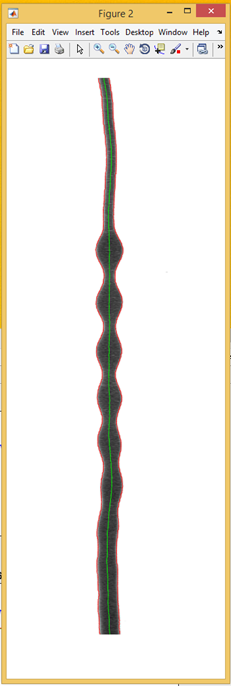
\includegraphics[scale=0.25]{./img/conduit1.png}
        \end{figure}
        \column{0.67\textwidth}
        \begin{figure}[H]
            \centering
            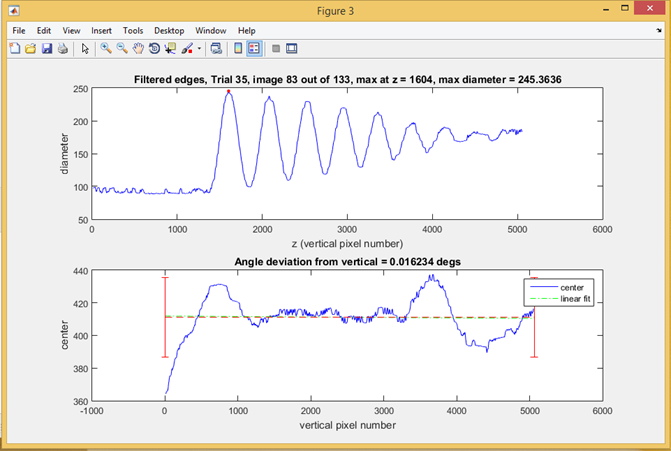
\includegraphics[scale=0.3]{./img/conduit2.png}
        \end{figure}
        Numeric data results from edge detection on images.
    \end{columns}
}

\frame{%
    \frametitle{What's the Issue?}
    \begin{columns}[c]
        \column{0.5\textwidth}
            \begin{itemize}
                \item How \textit{straight} is this conduit?
                \item Can we use data from this?
                \item Will our results be skewed?
                \item How do we quantify ``straightness''?
            \end{itemize}
            Again, this is a \textbf{Data Quality Problem}.
            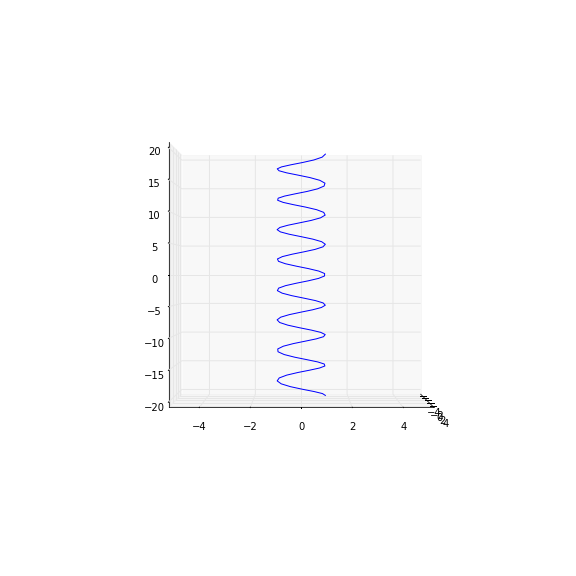
\includegraphics[scale=0.24]{./img/spiral_front.png}
        \column{0.5\textwidth}
            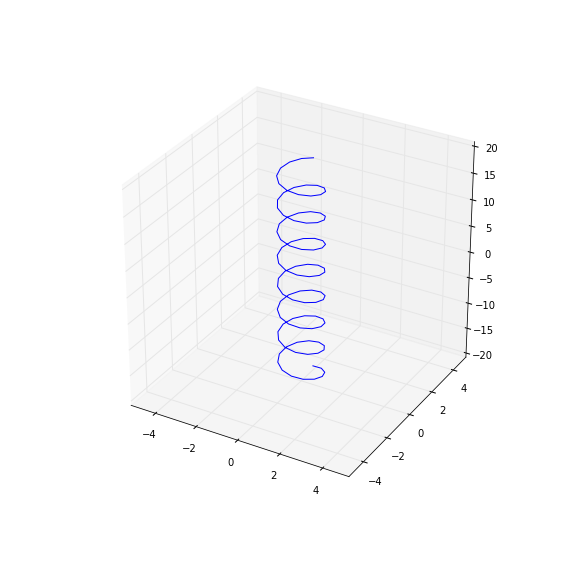
\includegraphics[scale=0.3]{./img/spiral.png}\\
    \end{columns}
}

\frame{%
    \frametitle{Algorithm}
    \begin{enumerate}
        \item Given some single-trial from edge detection on conduit image, find
            a smoothing fit.
        \item Repeat for all trials.
        \item Plot the \textit{Curvature} and \textit{Average Residual} of each
            smoothed trial fit on the plane.
        \item Use Classification Algorithms to determine the space of non-curvy
            lines, i.e.\ the space of good quality data.
    \end{enumerate}
}

\frame{%
    \frametitle{General Fit}
    \begin{columns}
        \begin{column}[c]{0.3\textwidth}
            By averaging the left and right edges of our axisymmetric conduit we
            can find the centerline.
        \end{column}
        \begin{column}[c]{0.7\textwidth}
            \begin{figure}[H]
                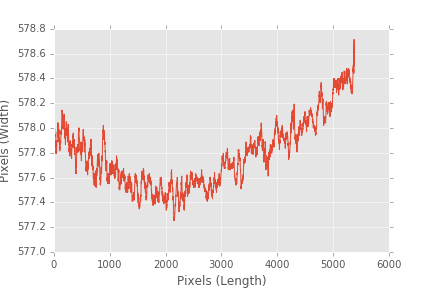
\includegraphics[scale=0.5]{./img/centerline.png}
            \end{figure}
        \end{column}
    \end{columns}
}

\frame{%
    \frametitle{Regression Model}
    \begin{columns}[T]
        \column{0.45\textwidth}
        We use the regression model
        \begin{align*}
            h(x) &= \beta_1 + \beta_2 x + \sum_{i=3}^n \beta_i f(x - x_i)
        \end{align*}
        where $f(y) = \beta e^{-{(sy)}^2}$.
        \begin{figure}[H]
            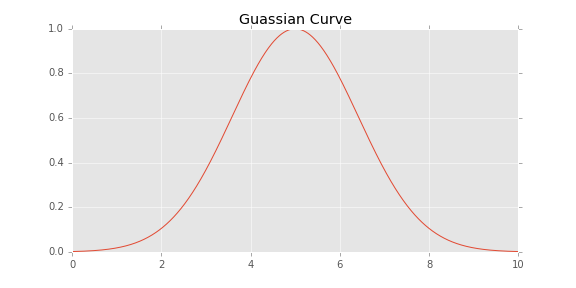
\includegraphics[scale=0.3]{./img/gaussian.png}
        \end{figure}
        \column{0.55\textwidth}
        \begin{figure}[H]
            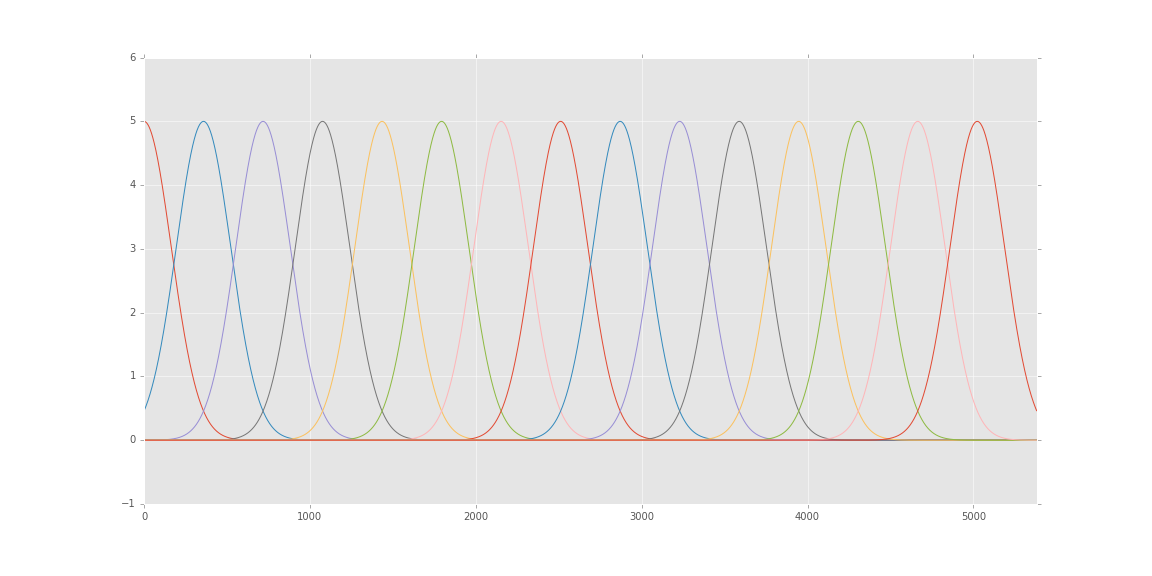
\includegraphics[height=2in, width=2.75in]{./img/gaussianoverlay.png}
        \end{figure}
    \end{columns}
}

\frame{%
    \frametitle{Example Fit}
    \begin{figure}[H]
        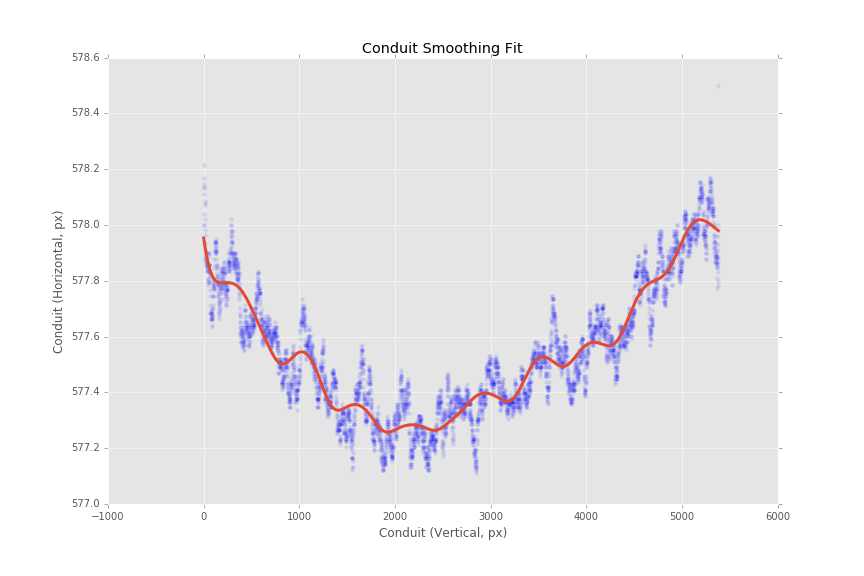
\includegraphics[scale=0.35]{./img/examplefit.png}
    \end{figure}
}

\frame{%
    \frametitle{Fit Parameter Determination}
    \begin{columns}[T]
        \column{0.4\textwidth}
        \begin{itemize}
            \item The shape parameter is how wide each gaussian is.
            \item The count parameter is how many gaussians we use in the
                regression.
            \item To find our parameters we examine every fit's residuals, take
                their mean, and the find the standard deviation of that set. Our
                ideal parameters have low standard deviation.
        \end{itemize}
        \column{0.6\textwidth}
        \begin{figure}[H]  % TODO: Source this
            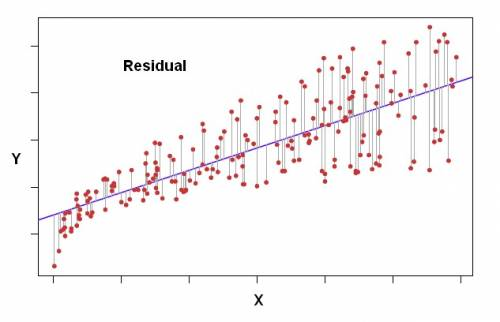
\includegraphics[scale=0.4]{./img/residuals.png}
        \end{figure}
        \begin{itemize}
            \item Examined using available data from the lab.
        \end{itemize}
    \end{columns}
}

\frame{%
    \frametitle{Sample Parameter Grid}
    \begin{figure}[H]
        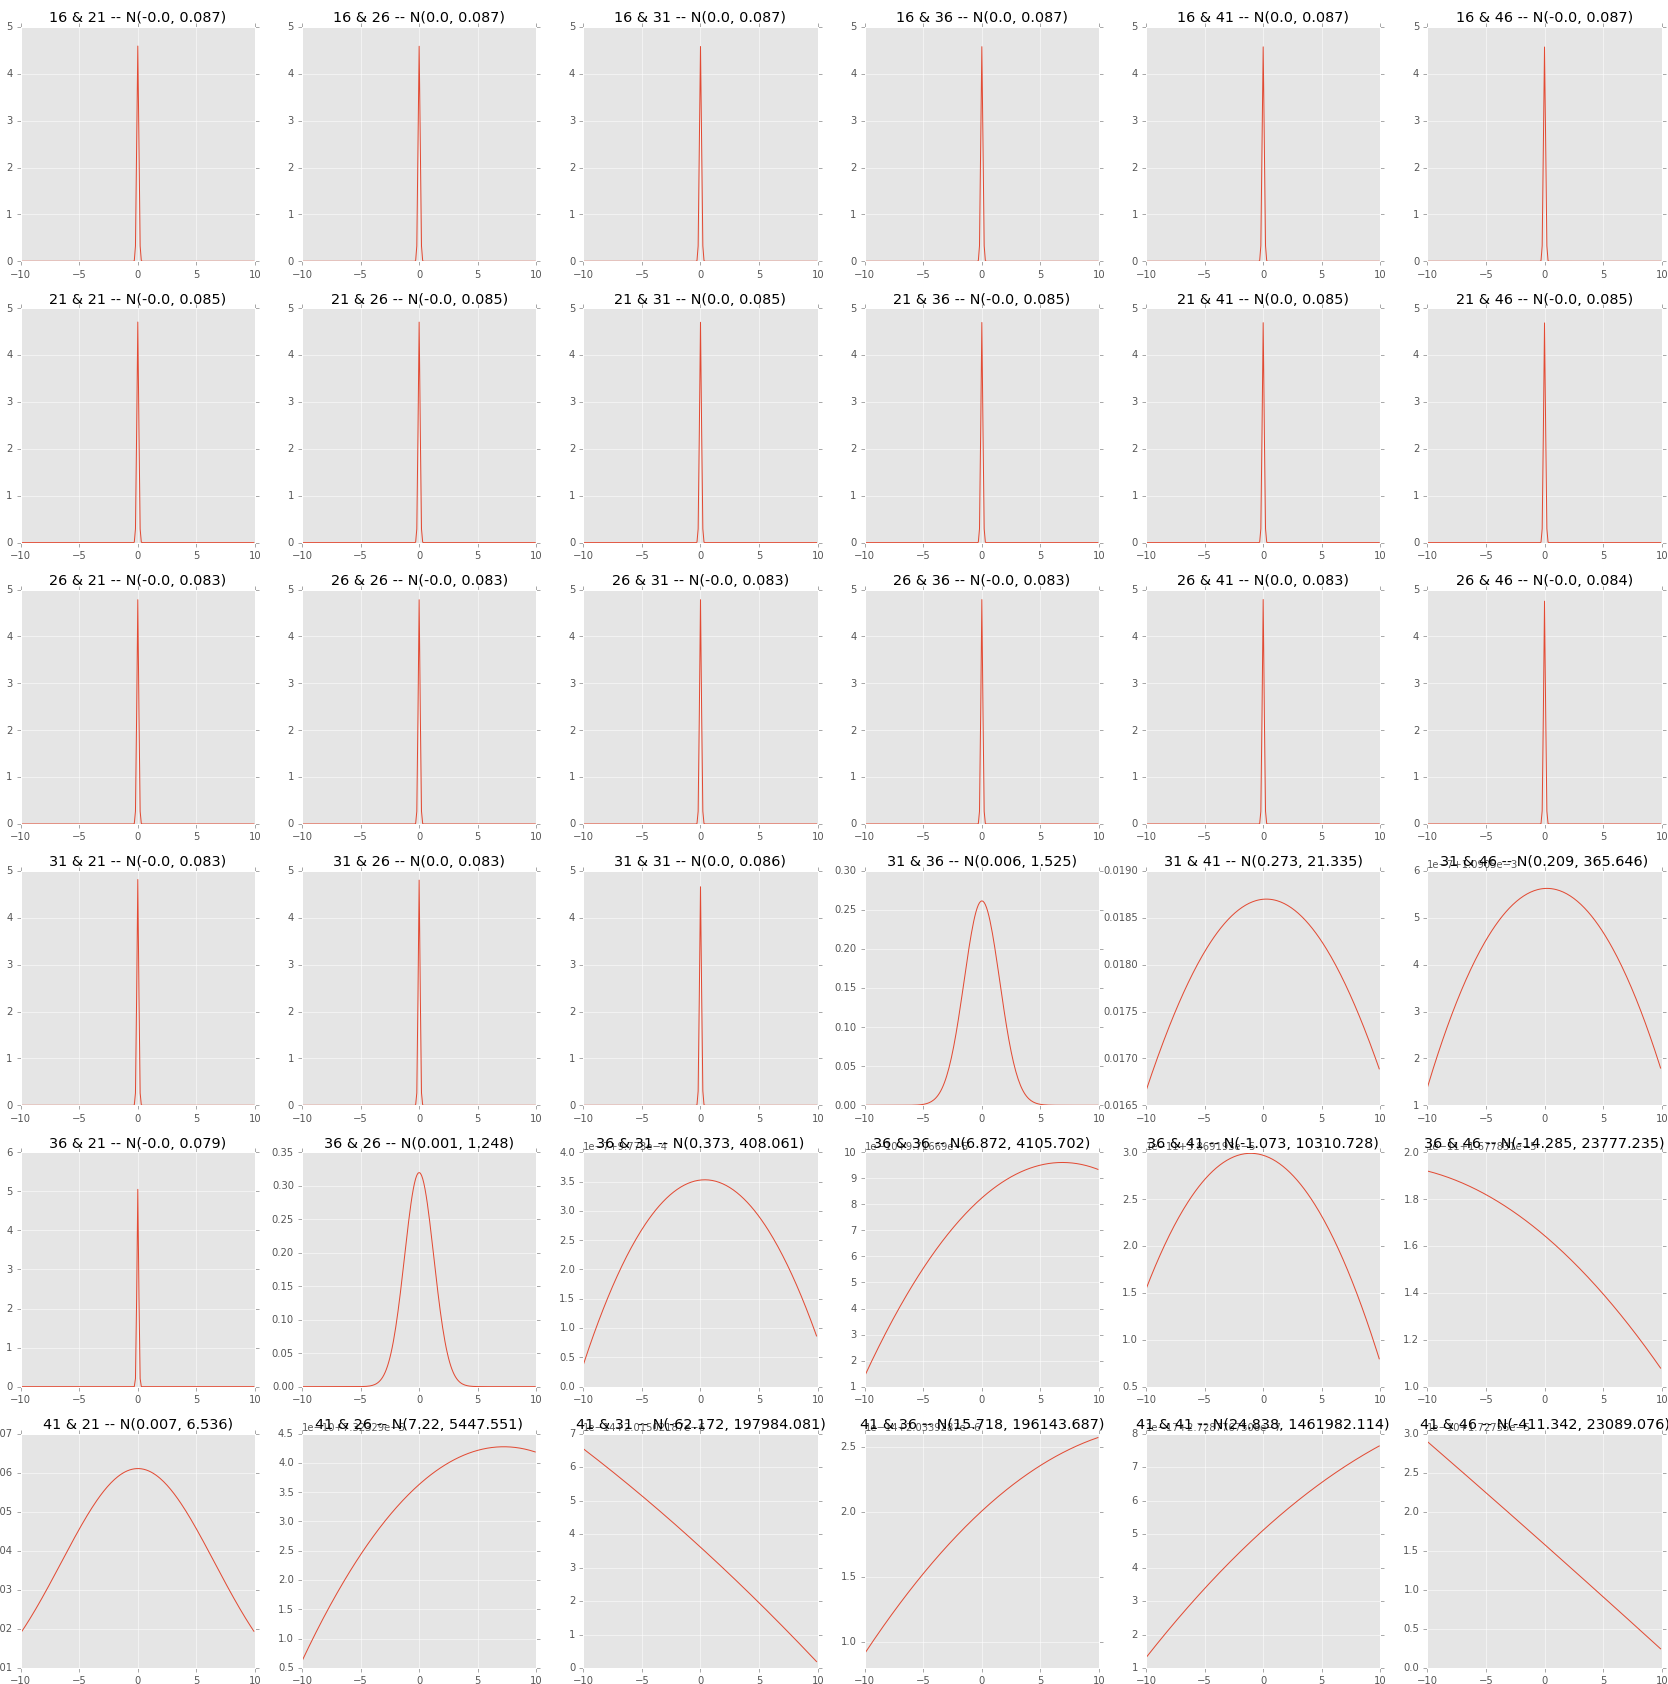
\includegraphics[scale=0.12]{./img/grid.png}
    \end{figure}
}

\frame{%
    \frametitle{Fit Comparison}
    \begin{figure}[H]
        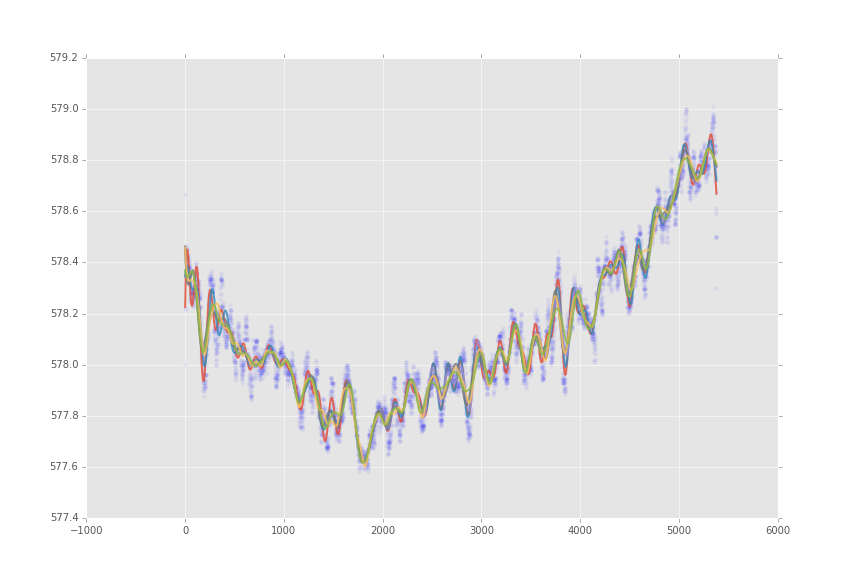
\includegraphics[scale=0.35]{./img/fitparam.png}
    \end{figure}
}

\frame{%
    \frametitle{Conduit Metrics}
    Now that we have a way to map our scattered points to a smooth line, we
    measure the quality of our collected data.
    \begin{itemize}
        \item Curvature - Based on second derivative
        \item Noise - Based on residuals. Included as if this is too high, it
            means the fit was poor, which can either indicate a blurry photo, or
            extreme curves.
    \end{itemize}
}

\frame{%
    \frametitle{Curvature}
    For this application, defined as
    \begin{align*}
        \frac{1}{n \cdot \text{scale}} \cdot
        \sqrt{\int_a^b {\left( s^{\prime\prime}(x)\right)}^2 \, dx}
    \end{align*}
    which is a non-dimensionalized number based on pixels and scaling factors.
}

\frame{%
    \frametitle{Noise}
    Residuals are defined as $y - \hat{y}$.
    \begin{figure}[H]  % TODO: Source this
        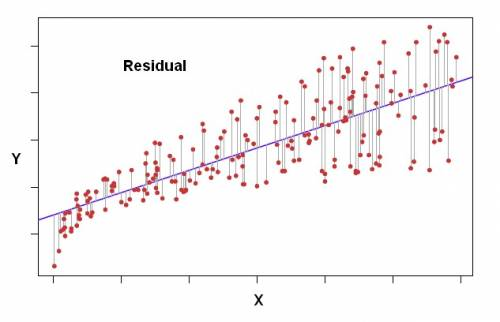
\includegraphics[scale=0.4]{./img/residuals.png}
    \end{figure}
    For this application, we define the noise as
    \begin{align*}
        \overline{\abs{y - \hat{y}}}.
    \end{align*}
}

\frame{%
    \frametitle{Plot}
    \begin{figure}[H]
        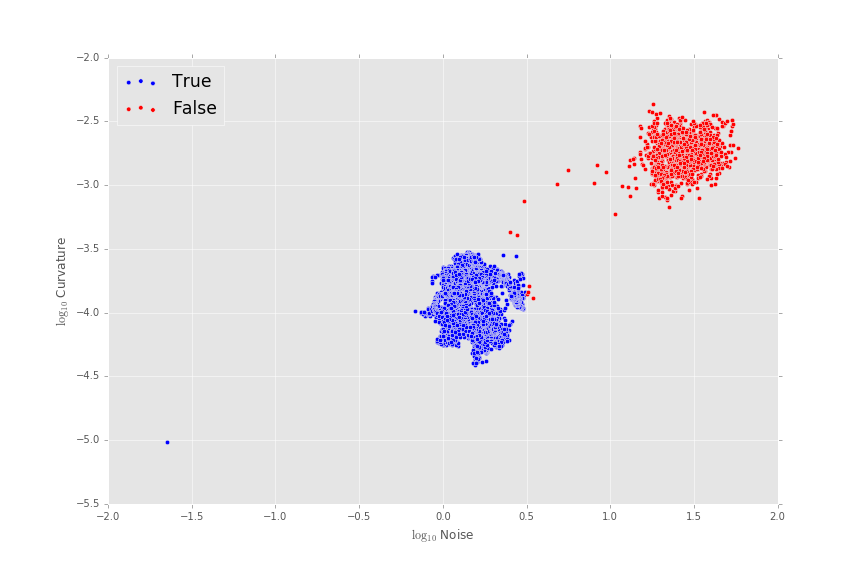
\includegraphics[scale=0.35]{./img/dataplot.png}
    \end{figure}
}

\frame{%
    \frametitle{Interpreting our Plot}
    \begin{columns}[T]
        \column{0.5\textwidth}
        \begin{itemize}
            \item How do we map this to our conduit?
            \item What do the clusters tell us?
            \item Where do we go from here?
        \end{itemize}
        \begin{figure}[H]
            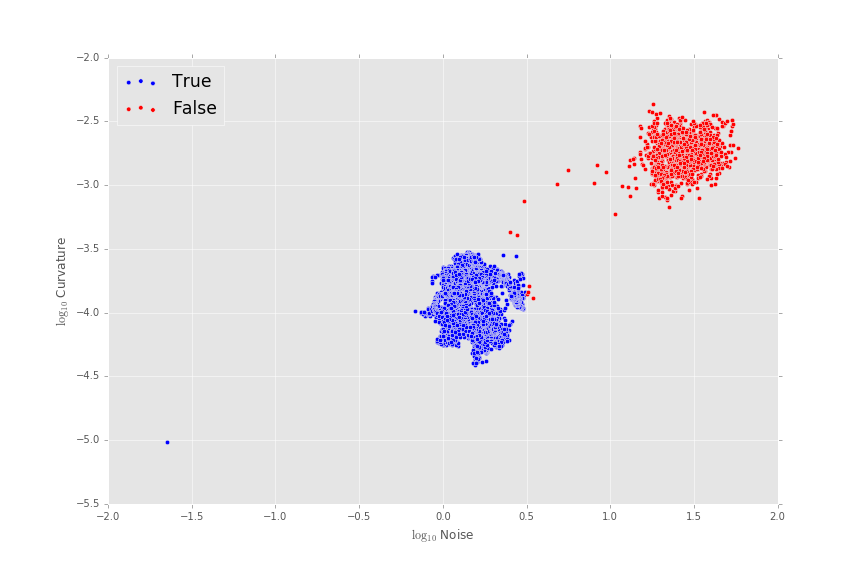
\includegraphics[scale=0.2]{./img/dataplot.png}
        \end{figure}
        \column{0.5\textwidth}
        \begin{figure}[H]
            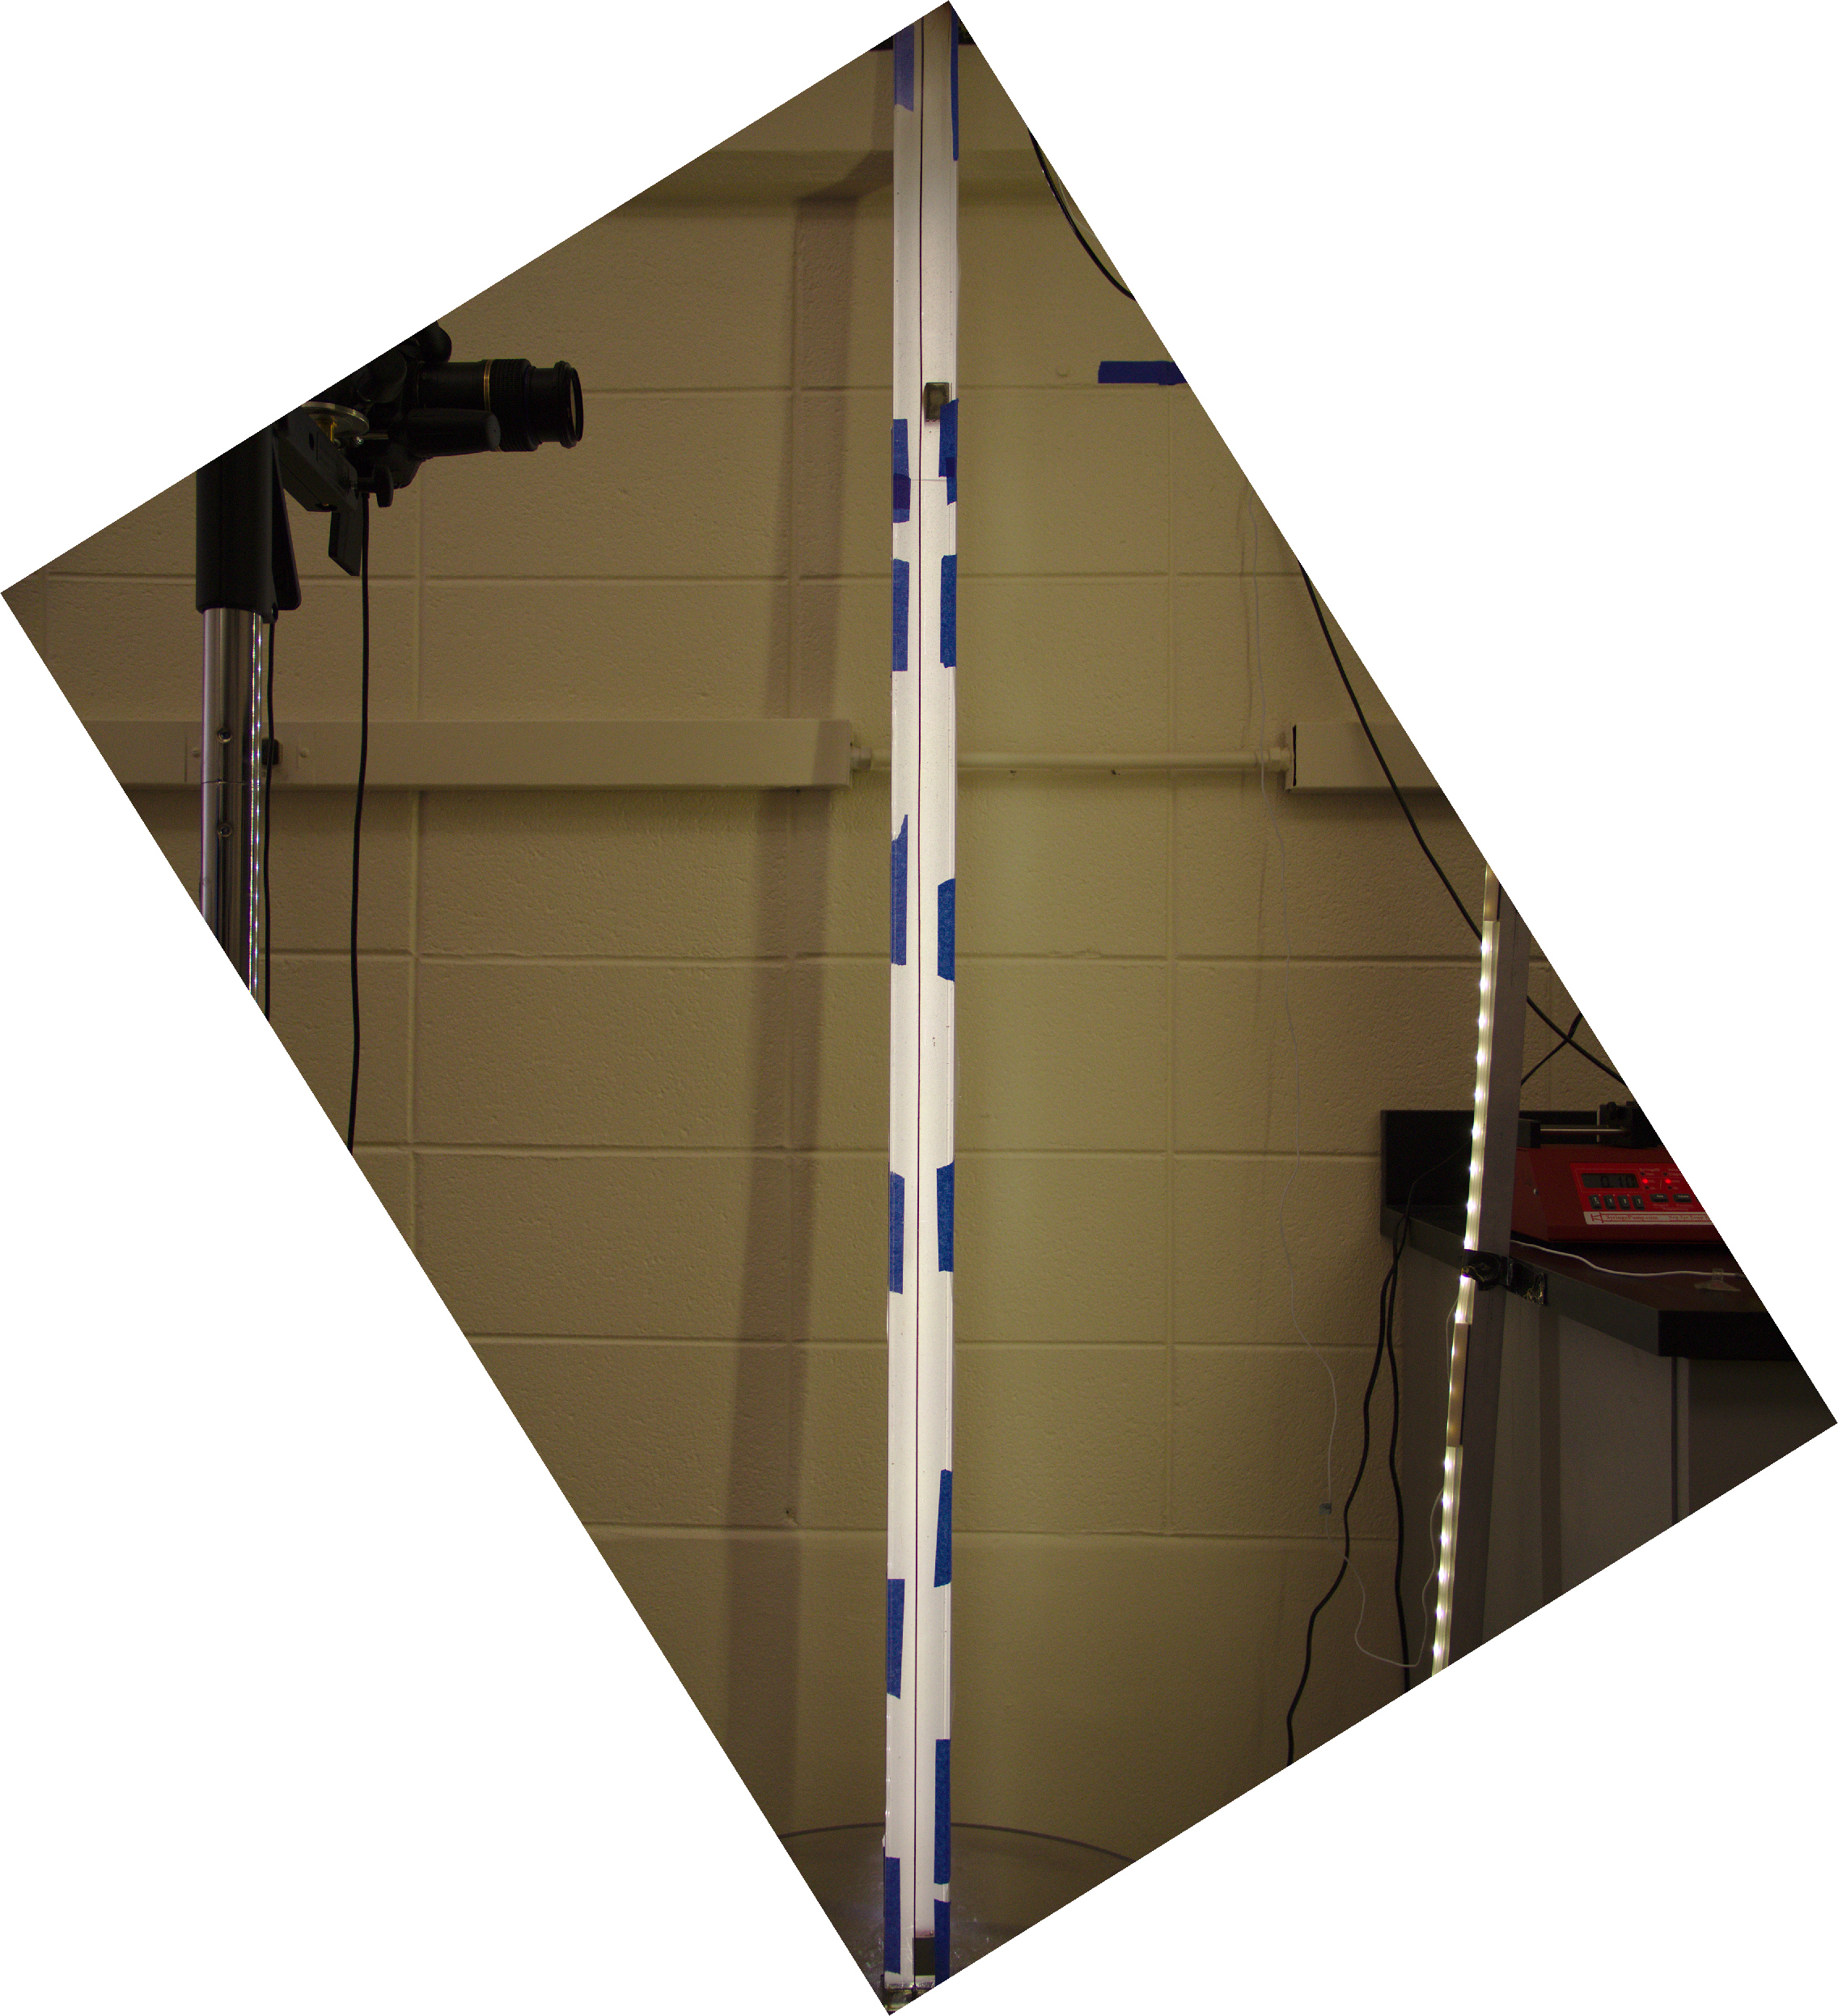
\includegraphics[scale=0.06]{./img/final.png}
        \end{figure}
    \end{columns}
}

\frame{%
    \frametitle{Example Fits}
    \begin{figure}[H]
        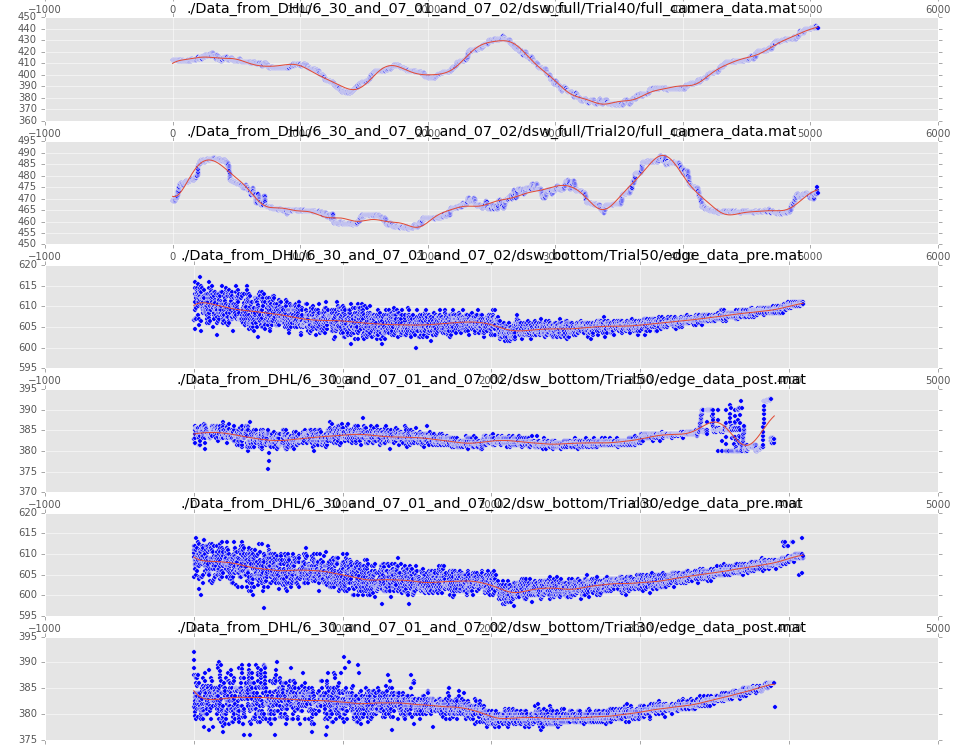
\includegraphics[scale=0.25]{./img/fits_small.png}
    \end{figure}
}

\frame{%
    \frametitle{A (Brief) Introduction to Machine Learning}
    \begin{itemize}
        \item For this problem, we need to use a subset of Machine Learning
            referred to as \textbf{classification}.
        \item Classification problems are those in which we need to sort a
            dataset into different categories.
        \item This perfectly describes our situation.
        \item These algorithms require a training and testing dataset.
        \item Our results will improve over time.
    \end{itemize}
}

\frame{%
    \frametitle{$k$-Nearest Neighbor Algorithm}
    $k$ nearby points ``vote'' on the class of the point in question.
    \begin{figure}[H]
        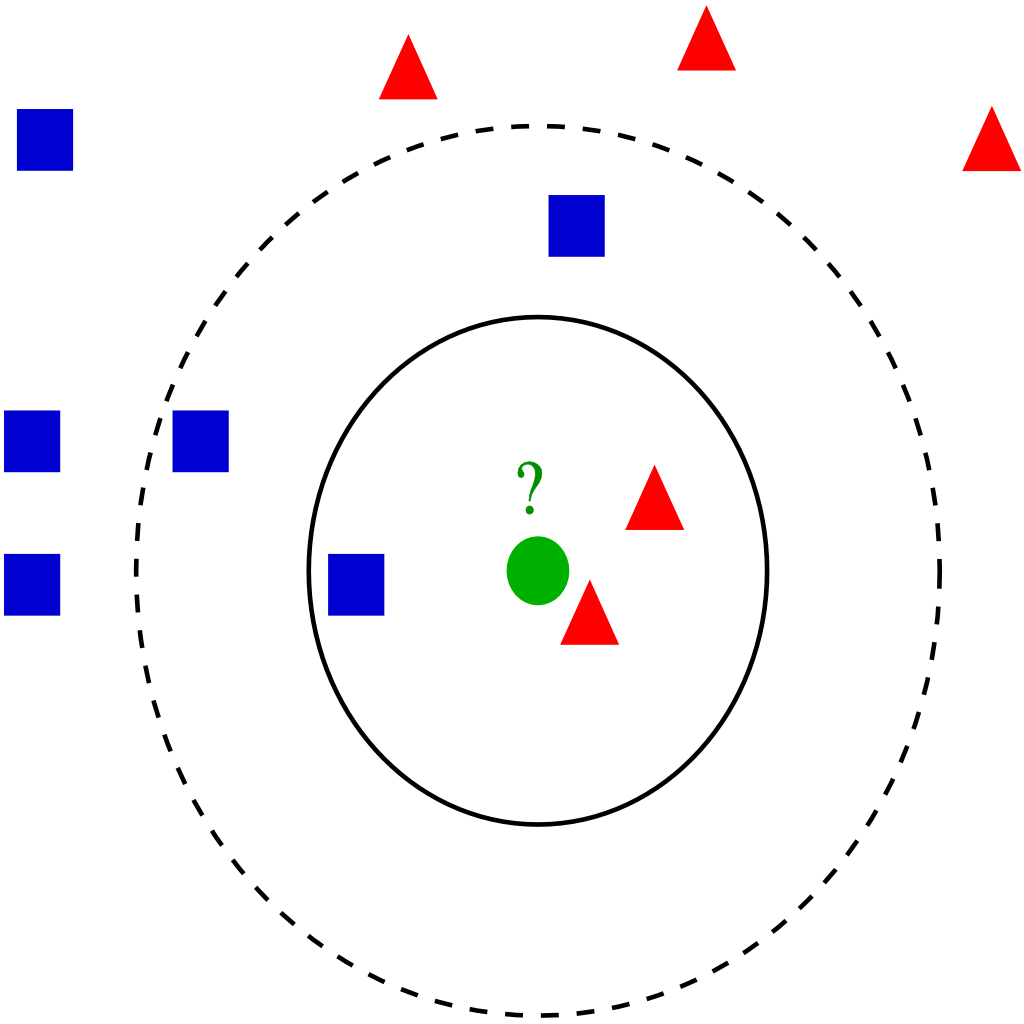
\includegraphics[scale=0.5]{./img/nnclass.png}
    \end{figure}
}

\frame{%
    \frametitle{Nearest Neighbor Application}
    \begin{figure}[H]
        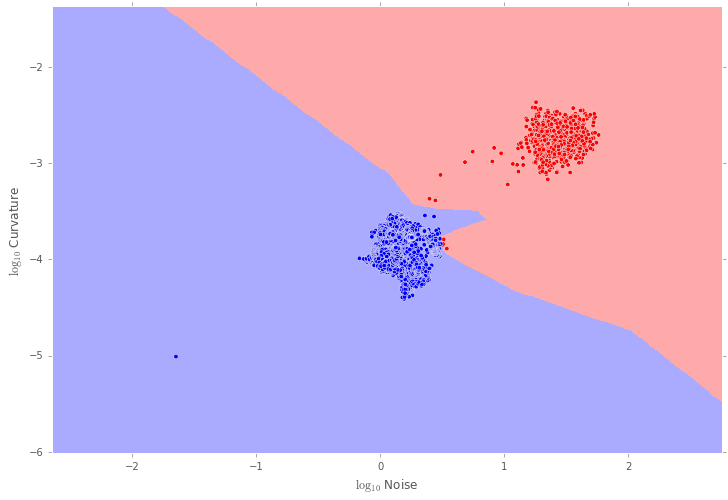
\includegraphics[scale=0.35]{./img/nn.png}
    \end{figure}
}

\frame{%
    \frametitle{Support Vector Machine Algorithm}
    Tries to find the optimal dividing line between classes.
    \begin{figure}[H]
        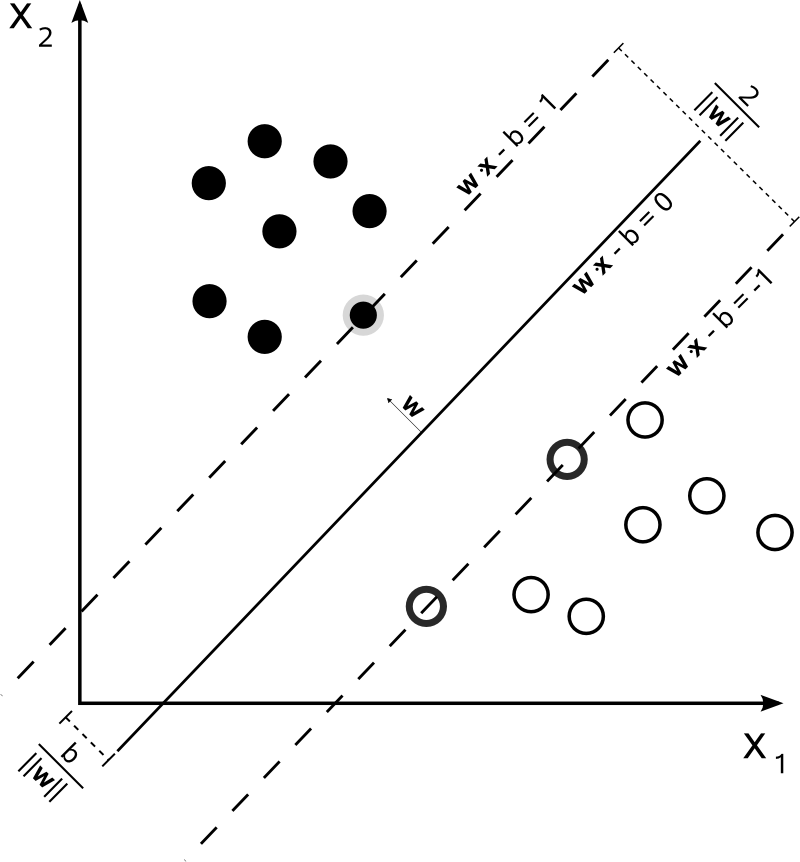
\includegraphics[scale=0.2]{./img/svm.png}
    \end{figure}
}

\frame{%
    \frametitle{Support Vector Machine with Linear Kernel}
    \begin{figure}[H]
        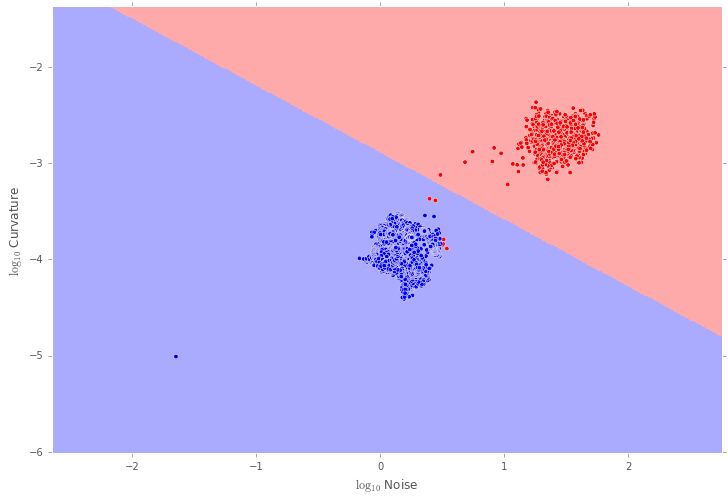
\includegraphics[scale=0.35]{./img/svm_linear.png}
    \end{figure}
}

\frame{%
    \frametitle{Support Vector Machine with RBF Kernel}
    \begin{figure}[H]
        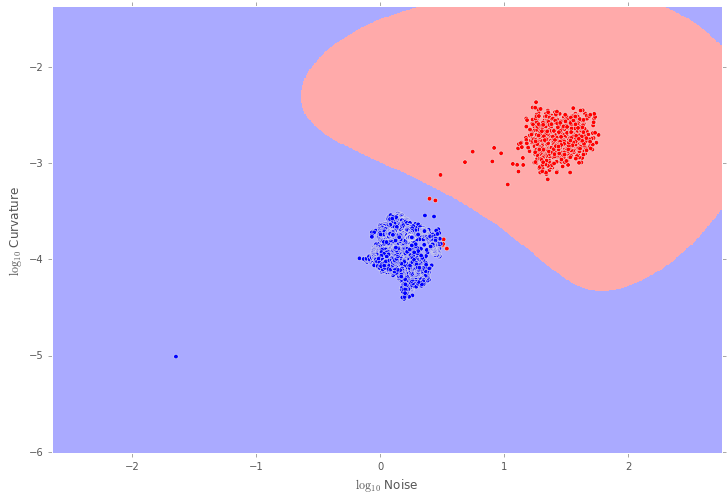
\includegraphics[scale=0.35]{./img/svm_rbf.png}
    \end{figure}
}

\frame{%
    \frametitle{Randomized Forest Algorithm}
    Creates a ``forest'' of decision trees and classifies based on mean result.
    \begin{figure}[H]
        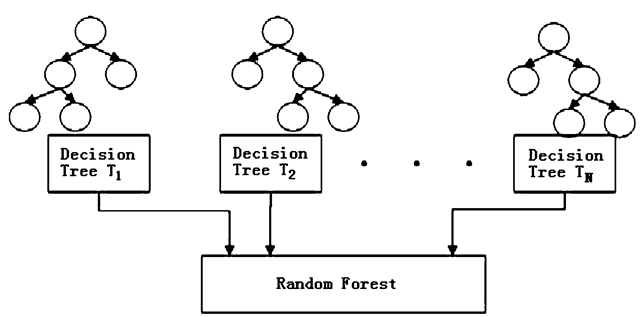
\includegraphics[scale=0.35]{./img/tree.png}
    \end{figure}
}

\frame{%
    \frametitle{Randomized Forest Application}
    \begin{figure}[H]
        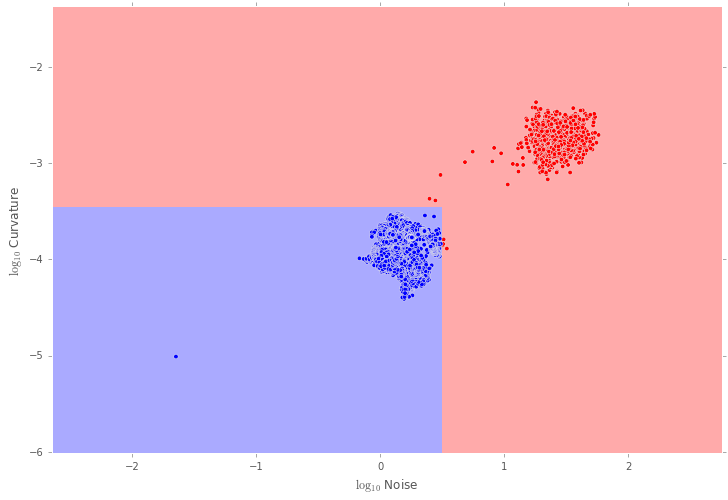
\includegraphics[scale=0.35]{./img/forest.png}
    \end{figure}
}

\frame{%
    \frametitle{So What?}
    \begin{itemize}
        \item \textbf{Poor quality data yields poor quality results.}
        \item We now can ensure good quality data.
    \end{itemize}
}

\frame{%
    \frametitle{Moving Forward}
    \begin{columns}[T]
        \column{0.5\textwidth}
        \begin{itemize}
            \item Now that we can ensure good quality data in our analysis we
                can move forward with some neat projects, like the Soliton Gas.
            \item A width problem instead of centerline.
            \item Where exactly is a specific soliton in a gas?
            \item Poisson?
        \end{itemize}
        \column{0.5\textwidth}
        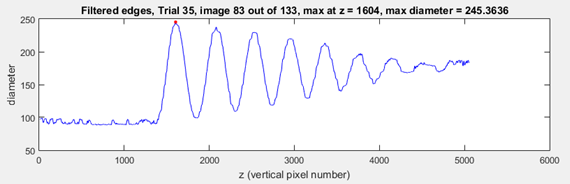
\includegraphics[scale=0.3]{./img/conduit3.png}\\
        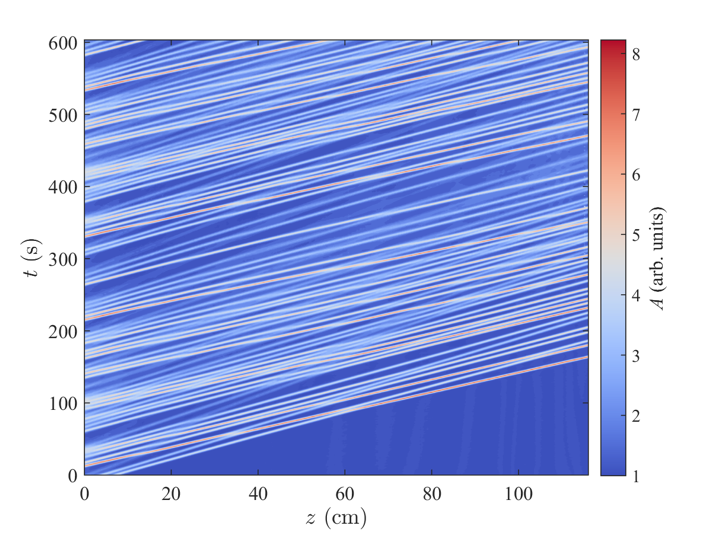
\includegraphics[scale=0.2]{./img/soliton_gas.png}
    \end{columns}
    \vspace{0.1cm}
    \movie[]{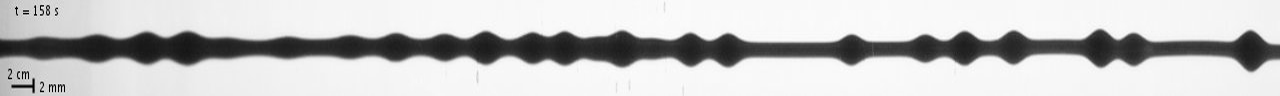
\includegraphics[scale=0.25]{./img/solitonmov.png}}{./img/soliton_gas.avi}
}

\frame{%
    \frametitle{Acknowledgements}
    \begin{itemize}
        \item Mark Hoefer
        \item Michelle Maiden
        \item Peter Wills
        \item Funded by NSF EXTREEMS-QED
    \end{itemize}
}
\end{document}
